\usecasebase{Prenotazione di un tavolo}
\label{usecase:Prenotazione di un tavolo}

\begin{figure}[h]
	\centering
	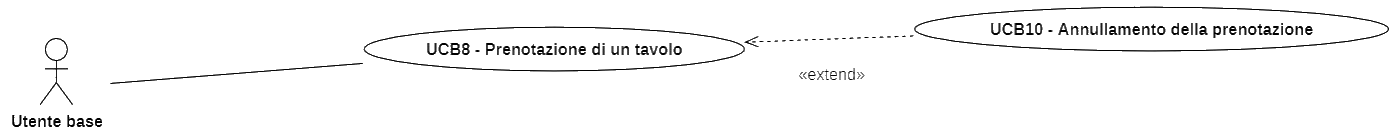
\includegraphics[width=0.9\textwidth]{./uml/UCB8-10.png} 
	\caption{Prenotazione di un tavolo}
	\label{fig:UCB8-10}
  \end{figure}

\begin{itemize}
	\item \textbf{Attore principale:} Utente base.
	\item \textbf{Precondizioni:}
	      \begin{itemize}
		      \item Un Utente base ha effettuato l'accesso al Sistema (vedi \autoref{usecase:Effettua accesso}).
		      \item Un Utente base visualizza la pagina di dettaglio di un ristorante (\autoref{usecase:Visualizzazione di un ristorante}).
	      \end{itemize}
	\item \textbf{Postcondizione:} L'Utente base ha confermato una prenotazione ed è tornato alla \textit{Home}.


	\item \textbf{Scenario principale:}
	      \begin{enumerate}
		      \item L'Utente base compila una \textit{form} di prenotazione;
		      \item L'Utente base seleziona il giorno e l'ora;
		      \item L'Utente base seleziona il numero di persone;
		      \item L'Utente base inserisce eventuali necessità: particolare bisogno di seggiolini per bambini oppure se è presente un commensale con qualche disabilità o problemi di movimento;
		      \item L'Utente base inserisce lo \textit{username} degli altri commensali che partecipano alla prenotazione (oppure la \textit{mail} se l'utente non è regisrato).
		            L'utente può anche decidere di non eseguire questo passaggio;
		      \item L'Utente base conferma la prenotazione;
		      \item Il Sistema crea un \textit{link} condivisibile con il resto dei commensali (vedi \autoref{usecase:Condivisione della prenotazione});
		      \item Il Sistema registra la prenotazione.

	      \end{enumerate}

	\item \textbf{Scenario secondario:}
	      \begin{itemize}
		      \item L'Utente base annulla la prenotazione (vedi
		            \autoref{usecase:Annullamento della prenotazione}).
		            \begin{enumerate}
			            \item L'Utente base annulla la prenotazione;
			            \item Il Sistema aggiorna la prenotazione;
		            \end{enumerate}
	      \end{itemize}
\end{itemize}

